\documentclass[12pt, a4paper, bibliography=totoc]{scrartcl}

% personal data
\date{\today}


% language
\usepackage{polyglossia}
\setmainlanguage{english}
\setotherlanguages{german}
\usepackage{microtype}
\usepackage{dcolumn}

\usepackage[style=numeric,
			natbib=true,
			backend=biber]{biblatex}		%Bibliographie
\usepackage[autostyle=true,
			 german=quotes]
			 {csquotes}					%Anführungszeichen
\usepackage{blindtext}


%math and theorems
\usepackage{amsmath}
\usepackage{amssymb}
\usepackage{amsopn}					%Matheoperatoren
\usepackage[amsmath,thmmarks,hyperref]{ntheorem}
\usepackage{mathtools}
\usepackage{mathdots}					%Punkte
\usepackage{dsfont}
\usepackage{upgreek}					%Griechische Buchstaben
\usepackage{bbm}						%Mengensymbol
\usepackage{physics}					%Physiksymbole
\usepackage{relsize}						%Größenangaben
\usepackage[separate-uncertainty,
			per-mode=symbol]
			{siunitx}					%Einheiten
%\usepackage{tikz}						%Zeichnen
\usepackage{upgreek}					%Griechische Buchstaben
\usepackage{enumitem}
\setlist{nolistsep}


%useful packages
%\usepackage{geometry}
\usepackage{xcolor}
\usepackage{graphicx}
\usepackage{float}
\usepackage{csquotes}
\usepackage{todonotes}
\usepackage{booktabs}
\usepackage{array}
\usepackage[labelfont=bf]{caption}
\usepackage{wrapfig}
\usepackage{enumitem}
%\usepackage{xr} % cross referencing
%\usepackage{titling}
%\usepackage{titlesec}
%\usepackage[Bjornstrup]
%			{fncychap}					%Kapitellayout


\setmainfont{Linux Libertine O}
\setsansfont{Linux Biolinum O}

\usepackage{scrhack}					%Verbesserung Pakete
\usepackage{xltxtra}						%fontec


\newcommand{\im}{\mathrm{i}}
\newcommand{\e}{\mathrm{e}}
\renewcommand{\pi}{\uppi}
\renewcommand{\epsilon}{\varepsilon}


\addbibresource{bibliography.bib}

%color settings
\definecolor{myred}{RGB}{196,19,47} 
\definecolor{myblue}{RGB}{0,139,139}


%appendix
\usepackage[toc,page]{appendix}

%killing indent
\setlength{\parindent}{0pt}
\usepackage{multicol}
\usepackage{siunitx}
\usepackage{hyperref}


\title{FP18 Atmospheric Trace Gases}
\author{Aaron Mielke \& Thomas Ackermann}
\date{\today}

\begin{document}

\begin{center}
	\makeatletter
	\thispagestyle{empty}
	\large{Fortgeschrittenen-Praktikum}	
	\hfill
    \large{Summer term 2019}
    \vspace{5mm}
	\rule{\textwidth}{0.2pt}
    \vfill
	\Huge\textbf{\@title} \\
	\vspace{10mm}
	\large{\@author} \\
	\normalfont
	\vfill	
	\makeatother
\end{center}

\normalsize
\newpage

\section*{Abstract}
This experiment was conducted in the scope of the advanced lab course in physics at the Heidelberg University. \\
The experiment was conducted in the week of the $8^\text{th}$ april, 2019.

\tableofcontents
\newpage
\begin{multicols}{2}
\section{Introduction}

\subsection{Zusammensetzung der Atmosphäre}
Die Atmosphäre der Erde besteht aus einer Mischung verschiedener Gase.
Tabelle \ref{fig:atm_comp} zeigt eine Liste der Hauptkomponenten.
\begin{center}
\begin{tabular*}{\linewidth}{c c c}
\toprule
Gas & Symbol & Rel. Anteil \\
\midrule
Stickstoff & \ch{N2} & $78.084 \%$ \\
    Sauerstoff & \ch{O2} & $20.942\%$ \\
    Argon & \ch{Ar} & 0.934 \% \\
    Kohlenstoffdioxid & \ch{CO2} & 358 \si{ppmv} \\

\bottomrule
\end{tabular*}
    \captionof{table}{Gase in der Atmosphäre} %\cite{atm_components}
    \label{fig:atm_comp}
\end{center}


\subsection{Messgrößen}
Die Konzentration eines Spurengases ist die Zahl der Moleküle pro Volumeneinheit.
Eine andere wichtige Größe ist die mixing ratio.
Sie gibt den relativen Anteil eines Spurengases im Vergleich zur Luftmenge an und wird mit \si{[ppm]} oder \si{[ppt]} angegeben. 

\subsection{DOAS}

    \textit{Differential Optical Absorption Spectroscopy} (DOAS) wird verwendet um die Konzentration eines bestimmten Spurengases in der Atmosphäre zu bestimmen - was das Ziel dieses Experimentes ist.
Das Haupprinzip ist das Folgende: 
    Man nimmt zwei Spektren auf, eines welches auf der Erde aufgenommen wurde (also mit absorption des Sonnenlichtes durch die Atmosphäre) und eines bei dem die Atmosphäre nicht präsent ist (Von Satelit aus aufgenommen.)
Jedes Gas absorbiert bestimmte Wellenlängen des Sonnenlichts.

\begin{center}
    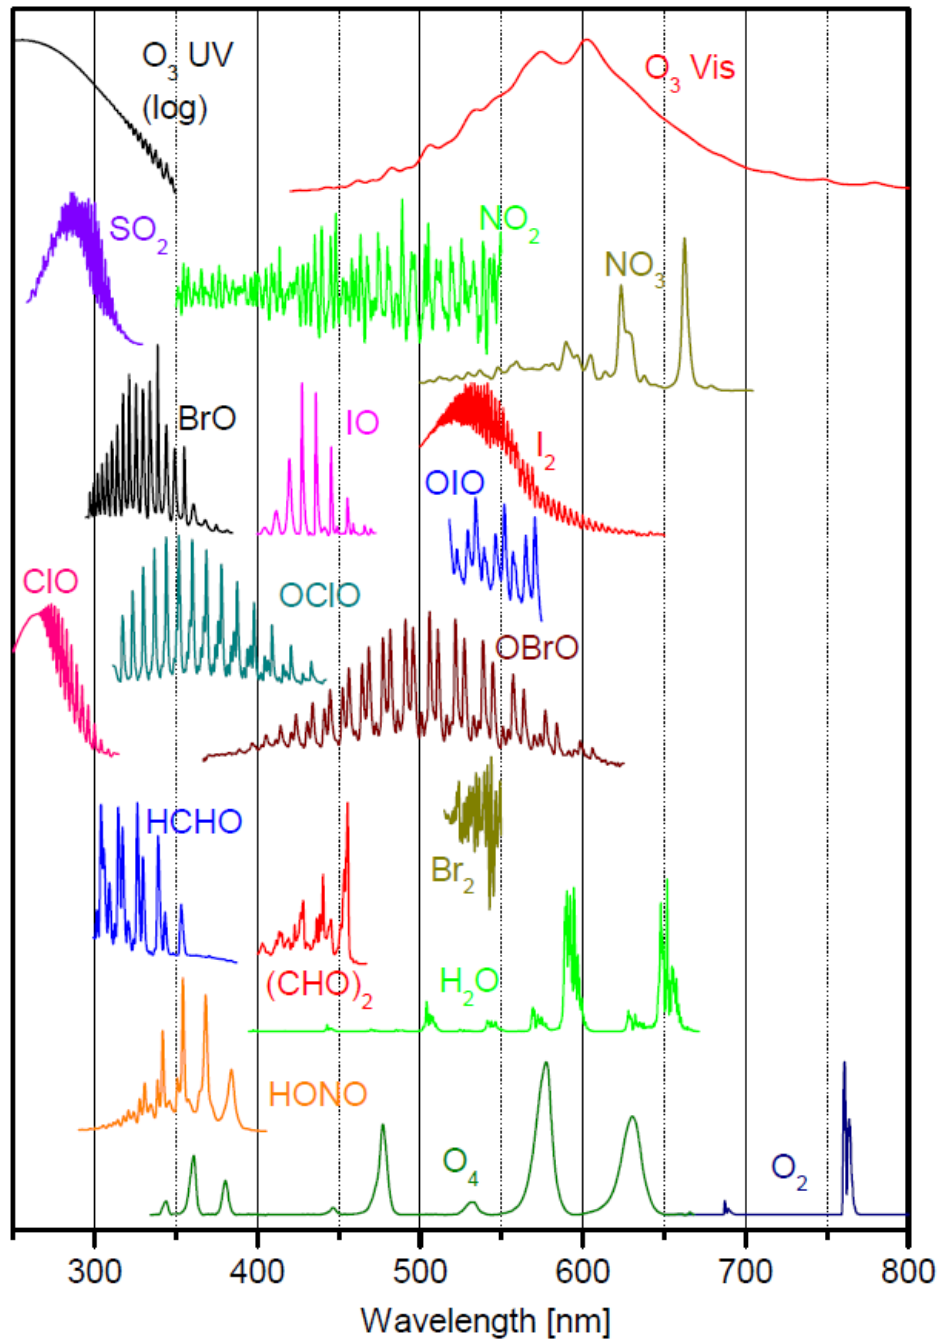
\includegraphics[width=0.7\linewidth]{fig/gas_spectra.png}
    \captionof{figure}{Charakteristische Linien verschiedener Gase}	
    \label{fig:gas_spectra}
\end{center}

Wenn nun zwei Spektren, wie beschrieben, aufgenommen werden 
können das charakteristische Verhalten der Gase daran erkannt werden dass die Intensitäten an manchen stellen kleiner sind.

Wenn man nun weiß welche charakteristika zu welchen Gasen gehören kann die Dichte des Gases in der Atmosphäre bestimmt werden.
In diesem Versuchsaufbau steht allerdings kein Satelit zur Verfügung so dass sich die frage stellt wie man an ein Sonnenspektrum ohne Atmosphäre kommt.
Die Lösung hier besteht daraus, dass Spektrum mit verschiedenen Winkeln aufgenommen wird und dann verglichen wird.
Die mittlere Weglänge die das Licht zurücklegt ist viel kürzer wenn genau im Zenit gemessen wird als bei anderen Winkeln.
Daher ist hier die Absorption durch Spurengase viel geringer sodass man einen ähnlichen Unterschied wie bei einem Sateliten erhält.

\subsubsection{Lambert-Beer Law}
    Die Intensität eines Lichtestrahls (einer Elektromagnetischen Welle) nimmt durch Streuung und Absorption ab, wenn es durch Materie propagiert (siehe Abbildung \ref{fig:lambert-beer}).
\begin{center}
    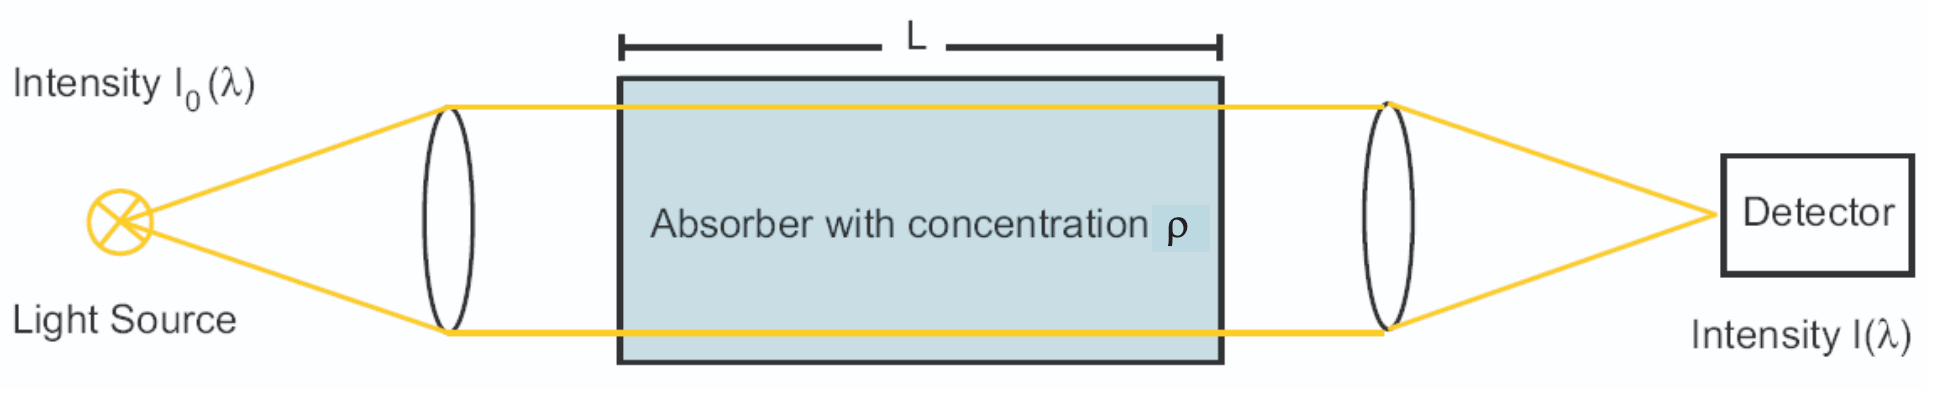
\includegraphics[width=\linewidth]{fig/lambert_beer.png}
    \captionof{figure}{Darstellung des Lambert-Beer Gesetzes}
	\label{fig:lambert-beer}
\end{center}

Die Größe des verlustes kann mithilfe des Lambert-Beer Gesetzes bestimmt werden.
    Sei $I_0 (\lambda)$ die Startintensität des Lichtstrahls, dann ist die Intensität $I(\lambda, L)$ nachdem der Lichtstrahl eine Länge $L$ der Mediums überwunden hat
    \begin{align}
        I(\lambda, L) = I_0 (\lambda) \exp \left( - \rho L \sigma (\lambda)\right) ,
    \end{align}
    wobei $\sigma (\lambda)$ der Absorptionswirkungsquerschnitt und $\rho$ die Konzentration des Spurengases ist.

\subsection{Kurzband Komponenten}
\subsubsection{Fraunhofer Referenzspektrum}

    \subsubsection{Spurengas Absorption}
    Die Hauptmessgröße des DOAS is die \textit{slant column density} ($SCD$ oder $S$)
    welche als die integrierte Dichte eines Spurengases $i$ entlang eines Lichtpfades der Länge $L$
    \begin{align}
        SCD = S_i (\lambda) = \int_0^{L(\lambda)} \rho_i (s) \dd s
    \end{align}

\subsection{Modifiziertes Lambert-Beer Gesetz}

Wenn man nun diese Effekte mit einbezieht, so kann man ein neues modifiziertes Lambert-Beer Gesetz austellen.
\begin{align*}
    I(\lambda, L) = & I_0 (\lambda) \exp \left( -R ( \lambda ) - \sum_i \sigma_i (\lambda)
    S_i (\lambda) \right) \times \\
    & \exp \left[ - L \left( \sigma_{i0} (\lambda) \rho_o + \epsilon_R (\lambda) + \epsilon_M (\lambda) \right) \right]
\end{align*}
Die erste Exponentialfunktion beinhaltet alle Kurzband Effekte und die zweite alle Breitband Effekte.
Wenn man das modifizierte Lambert-Beer Gesetz nun nach $\log \frac{I}{I_0}$ umformt erhält man die optische Dichte $\tau$:
\begin{align}
\tau &= \log \frac{I}{I_0} \\
    &= - R(\lambda) - \sum_i \sigma_i (\lambda) S_i (\lambda) - \sum_k b_k \lambda^k
\end{align}
wobei das Polynom $\sum b_k \lambda^k$ für die Breitband Effekte zuständig ist.


\section{Versuchsdurchführung}



\subsection{Software kennenlernen}

Während des Versuches wurde das Programm DOASIS verwendet um die Spektren aufzunehmen und später die Fits durchzuführen.\\
Zu Beginn wurden bei denen die Messzeit und die Anzahl der Scans variiert wurde.

\begin{center}
	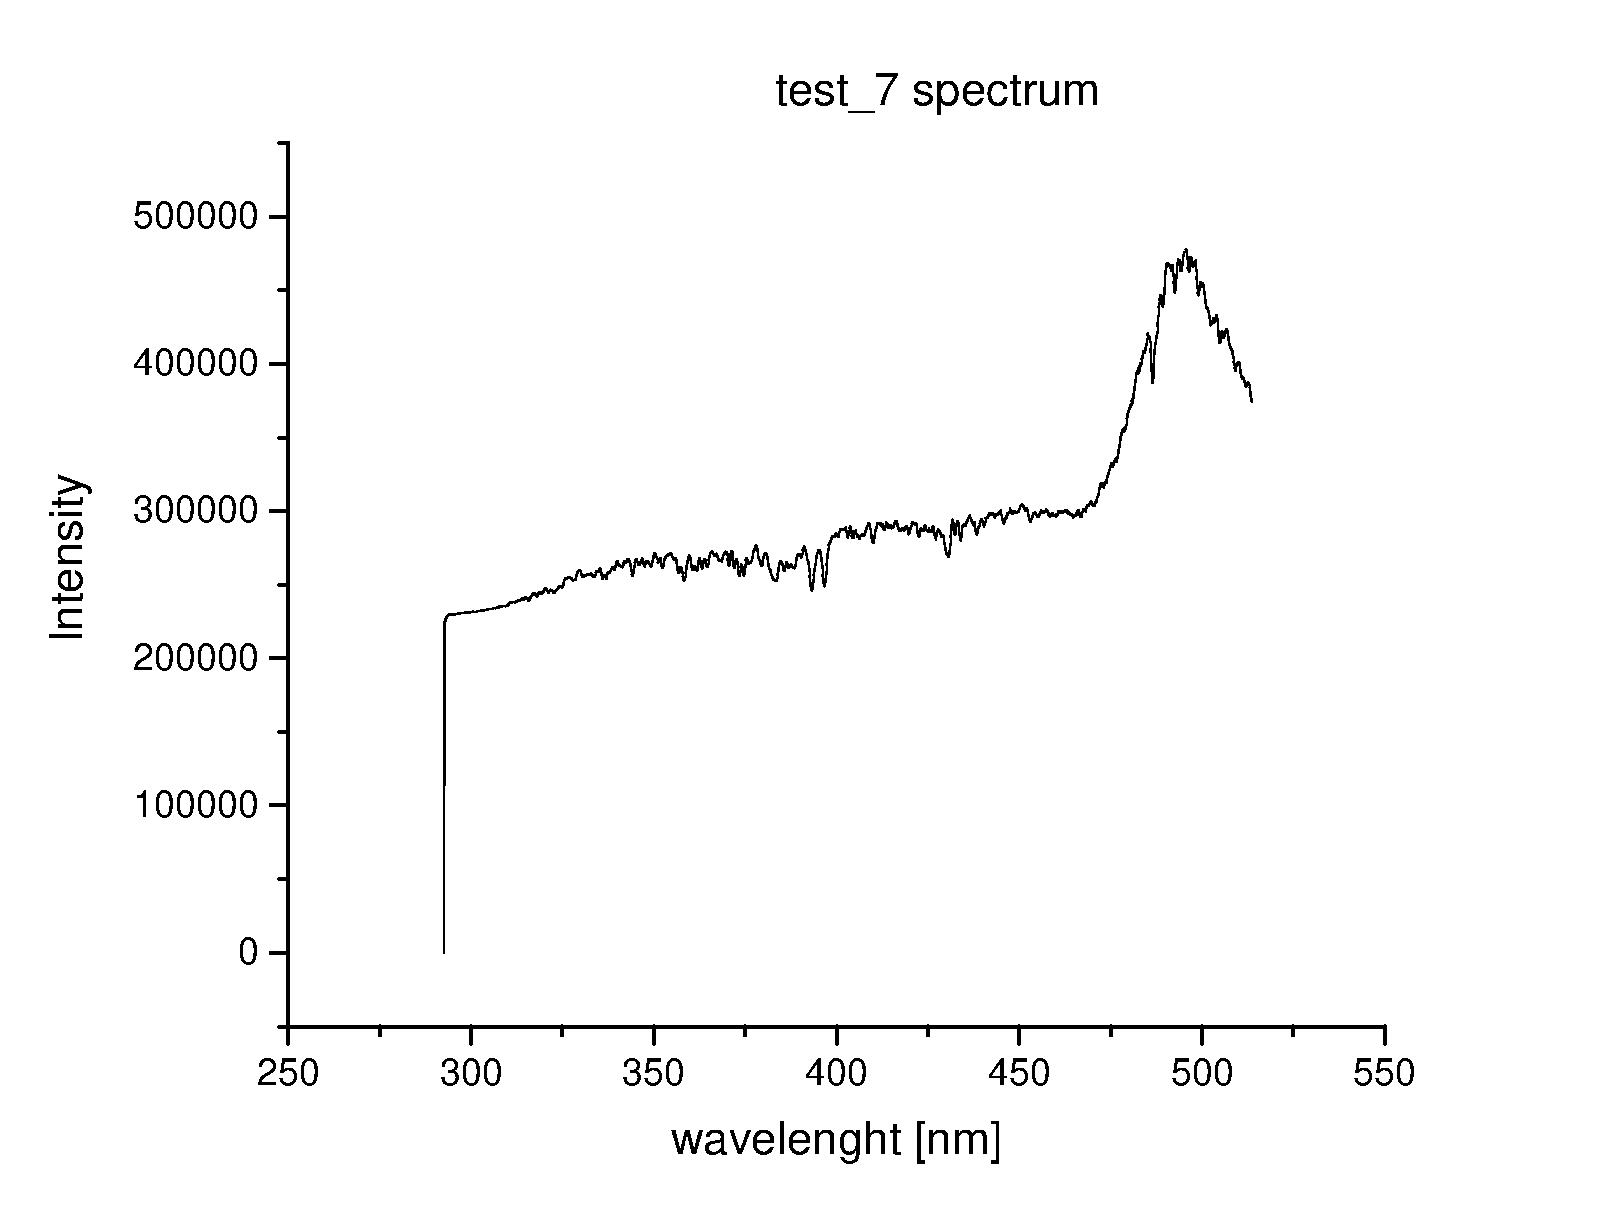
\includegraphics[width=\linewidth]{fig/test_7_spectrum.pdf}
    \captionof{figure}{Test Spektrum}
	\label{fig:test_spectrum}

\end{center}

\subsection{Charakterisierung der Messinstrumente}
Es gibt zwei Haupteffekte die Ungenauigkeiten bei der Messung verursachen können.
Durch Brownsche Bewegung in den Kabeln wird ein kleiner elektrischer Strom erzeugt, den man auch Dunkelstrom nennt.
Um die Größenordnung des Dunkelstromes einzuschätzen werden einminütige Messungen durchgeführt, bei denen die Kamera abgedeckt ist.
Die CCD-Kameras haben außerdem ein Offset, welcher durch viele kurze Messungen bestimmt werden kann.\\
Dunkelstrom und Offset müssen bei jedem folgenden Spektrum abgezogen werden.
Die Messung des Offsets wurde als erstes Durchgeführt. 
Hierbei wurden 20000 Messungen mit jeweils $3$ \si{ms} Messzeit durchgeführt.
    Anschließend wurde der Dunkelstrom bei verschiedenen Messzeiten gemessen (siehe Abbildung \ref{fig:dark_current}).
\begin{center}
	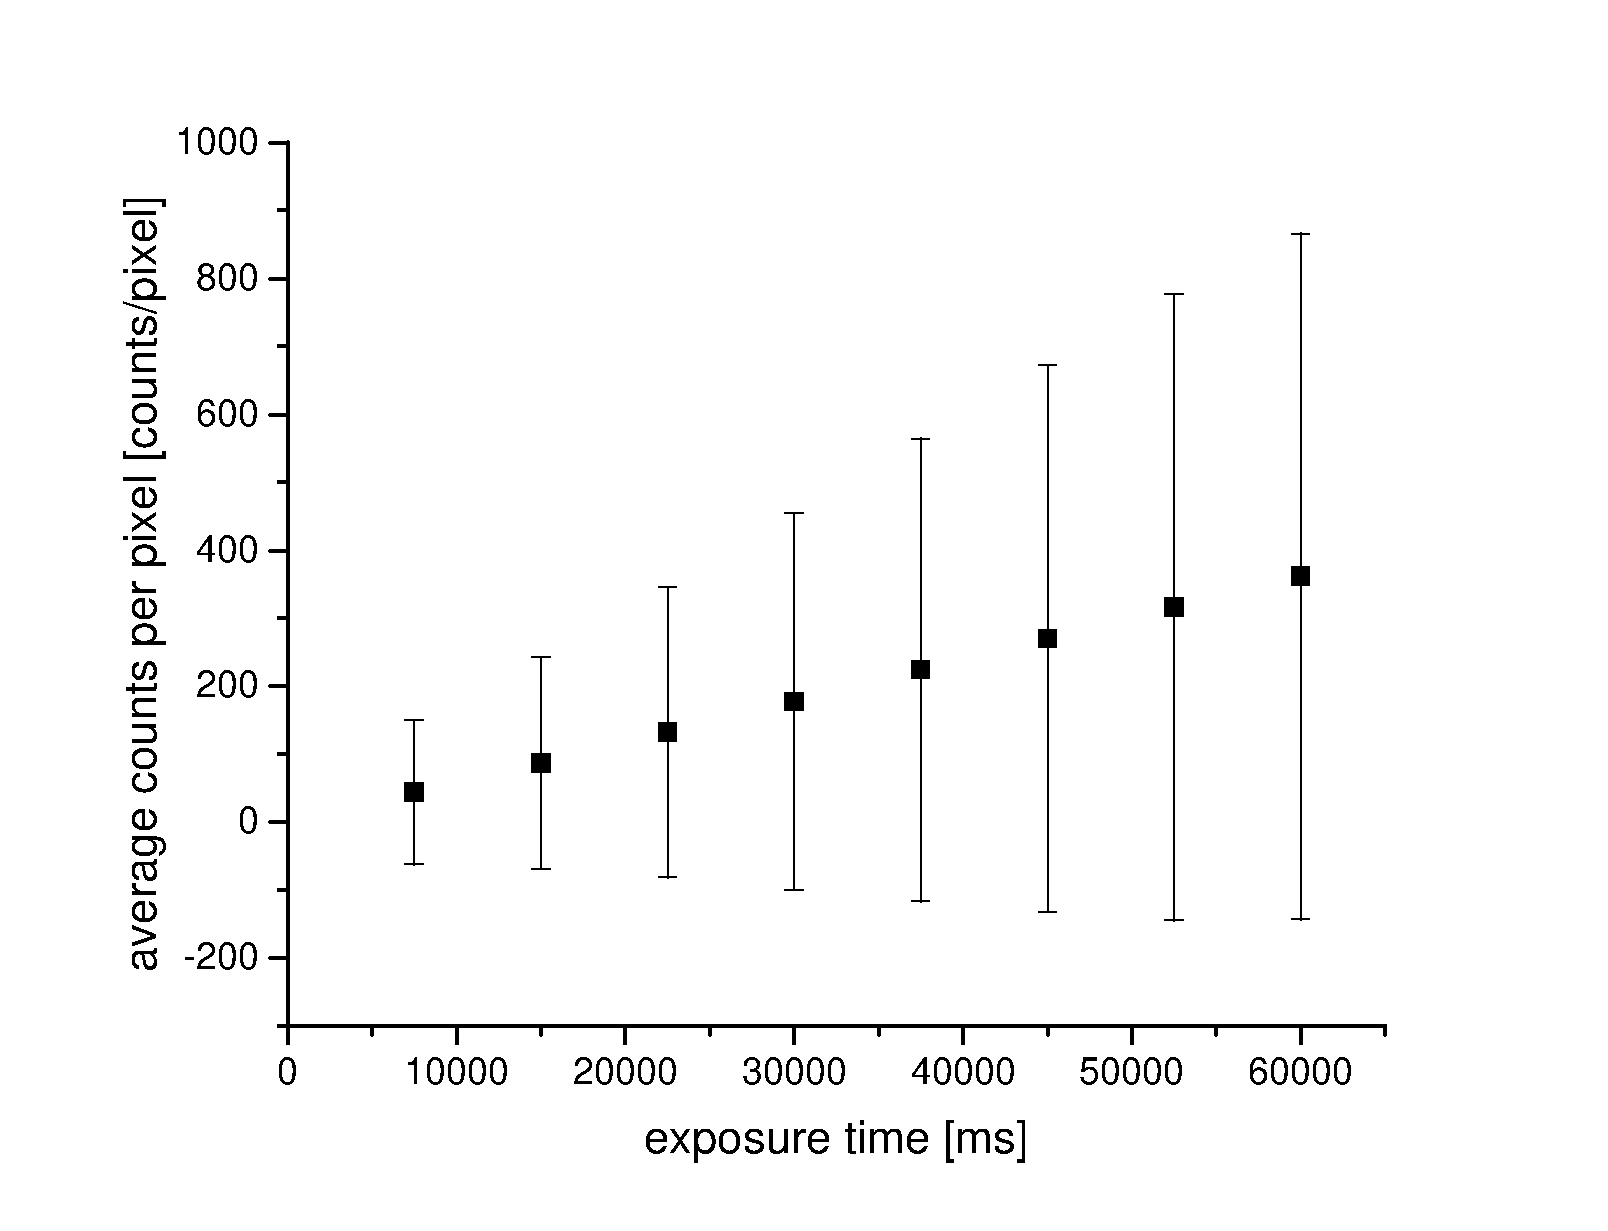
\includegraphics[width=\linewidth]{fig/dark_current_exposure_time_plot.pdf}
    \captionof{figure}{Abhängigkeit des Dunkelstromes von der Messzeit}
	\label{fig:dark_current}
\end{center}

\subsection{Labormessungen}
Mithilfe eines Literaturspektrums kann ein Vergleichsspektrum generiert werden. 
Die verwendeten Literaturspektren haben allerdings unterschiedliche Auflösungen und daher muss man diese entsprechend skalieren.
Dies kann mithilfe einer Faltung erledigt werden.
Die Faltung einer Funktion $f$ mit einer Funktion $g$ ist definier als

    \begin{align}
(f \ast g) (x) := \int f(y) g(x-y) \dd y .
    \end{align}
Die Faltung sorgt zusätzlich dafür, dass das Spektrum geglättet wird.
Wellenlänge die außerhalb des Bereiches der Messgeräte liegt werden duch die Faltung abgeschnitten.\\


\subsection{Atmosphärische Messungen}

\subsection{Multi Axis DOAS}



\end{multicols}
\end{document}

